\documentclass{article}
\usepackage{tikz, comment}
\usepackage{pifont}
\usepackage{fontspec}
\usetikzlibrary{arrows, decorations.markings, decorations.pathreplacing}
\begin{comment}
:Title: Not defined yet
:Slug: No name yet

Description Here.........
\end{comment}
\begin{document}\centering

\def\a{2.75}
\def\b{5.25}

\begin{tikzpicture}[>=latex,xscale=.5*0.5, yscale=.5*0.5][font=\sf\small] 
    %Circles 
   \foreach \r in {1, 1.5, 3, 5, 7, 9}
      \draw[thin, color=gray!40] (0,0) circle (\r);
    \foreach \r in {2, 4, 6, 8}
      \draw[thick, color=gray!40] (0,0) circle (\r);   
    %1° Rays
    \foreach \a in {0, 1,...,359}
      \draw[] (\a:9.7) -- (\a:10);
    %5° Rays
    \foreach \a in {0, 5,...,359}
      \draw[] (\a:9.5) -- (\a:10);      
    %15° Rays
    \foreach \a in {0, 15,...,359}
      \draw[thick, color=gray!40] (\a:1.5) -- (\a:10); 
    %30° Rays
    \foreach \a in {0, 30,...,359}
      \draw[thick, color=gray!40] (0, 0) -- (\a:10);
    %Radius labels (background filled white)
    \foreach \r in {{5.25-2.75}}
      \draw[] ({\r},0) node[inner sep=1pt,above=1pt,rectangle,fill=white, xshift=6, scale=0.5] {$b-a$};
    \foreach \r in {{5.25+2.75}}
      \draw[] ({\r},0) node[inner sep=1pt,above=1pt,rectangle,fill=white, xshift=6, scale=0.5] {$b+a$};
    %Main rays
    \foreach \a in {0, 90,...,359}
      \draw[very thick, color=gray!40] (0, 0) -- (\a:10);
    %Angle labels  
    \foreach \a in {0, 15,...,359}
      \draw (\a: 10.75) node[scale=0.5] {$\a^\circ$};
    %Central point
    \draw[fill=red] (0,0) circle(0.7mm/0.5);

\clip (0, 0) circle (10);

\foreach \p/\q in {0/{2*pi}}    		
\draw[purple, thick, samples=100, smooth, domain=\p:\q, variable=\t] 
		plot ({(2.75+5.25*cos(\t r))*cos(\t r)}, {(2.75+5.25*cos(\t r))*sin(\t r)});

\draw[teal, dashed] (0, 0) -- ({10*cos((rad(acos(-(\a)/(\b)))) r)}, {10*sin((rad(acos(-(\a)/(\b)))) r)}) node[right, pos=0.8, fill=white, xshift=3, scale=0.5] {$\theta=\arccos(-\frac{a}{b})$};
\draw[teal, dashed] (0, 0) -- ({10*cos((2*pi-rad(acos(-(\a)/(\b)))) r)}, {10*sin((2*pi-rad(acos(-(\a)/(\b)))) r)}) node[right, pos=0.8, fill=white, xshift=3, scale=0.5] {$\theta=2\pi- \arccos(-\frac{a}{b})$};

\foreach \x in {{\b-\a}, {\b+\a}}
	\draw (\x, {2pt/(0.5)}) -- (\x, {-2pt/(0.5)});
	
\foreach \y in { {\a} }
\draw ({2pt/(0.5)}, \y) -- ({-2pt/(0.5)}, \y) node[anchor=east, scale=0.5] {$a$};

\end{tikzpicture}\hskip1cm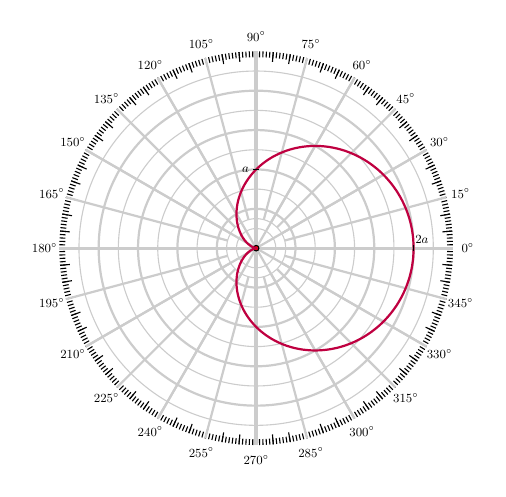
\begin{tikzpicture}[>=latex,xscale=.5*0.5, yscale=.5*0.5][font=\sf\small] 
    %Circles 
   \foreach \r in {1, 1.5, 3, 5, 7, 9}
      \draw[thin, color=gray!40] (0,0) circle (\r);
    \foreach \r in {2, 4, 6, 8}
      \draw[thick, color=gray!40] (0,0) circle (\r);   
    %1° Rays
    \foreach \a in {0, 1,...,359}
      \draw[] (\a:9.7) -- (\a:10);
    %5° Rays
    \foreach \a in {0, 5,...,359}
      \draw[] (\a:9.5) -- (\a:10);      
    %15° Rays
    \foreach \a in {0, 15,...,359}
      \draw[thick, color=gray!40] (\a:1.5) -- (\a:10); 
    %30° Rays
    \foreach \a in {0, 30,...,359}
      \draw[thick, color=gray!40] (0, 0) -- (\a:10);
    %Radius labels (background filled white)
    \foreach \r in {{4+4}}
      \draw[] ({\r},0) node[inner sep=1pt,above=1pt,rectangle,fill=white, xshift=3, scale=0.5] {$2a$};
    %Main rays
    \foreach \a in {0, 90,...,359}
      \draw[very thick, color=gray!40] (0, 0) -- (\a:10);
    %Angle labels  
    \foreach \a in {0, 15,...,359}
      \draw (\a: 10.75) node[scale=0.5] {$\a^\circ$};
    %Central point
    \draw[fill=red] (0,0) circle(0.7mm/0.5);

\clip (0, 0) circle (10);

\foreach \p/\q in {0/2*pi}    		
\draw[purple, thick, samples=100, smooth, domain=\p:\q, variable=\t] 
		plot ({(4+4*cos(\t r))*cos(\t r)}, {(4+4*cos(\t r))*sin(\t r)});

\foreach \x in {{2*4}}
\draw (\x, {2pt/(0.5)}) -- (\x, {-2pt/(0.5)});

\foreach \y in {4}
\draw ({2pt/(0.5)}, \y) -- ({-2pt/(0.5)}, \y) node[anchor=east, scale=0.5] {$a$};
    
\end{tikzpicture}
\end{document}